\documentclass[11pt]{beamer}

% packages
\usepackage[utf8]{inputenc}
\usepackage[T1]{fontenc}

\usepackage{graphicx}

% Beamer theme
\usetheme{Boadilla} % other interesting built-in: Boadilla, CambridgeUS (if we want sections in header), Pittsburgh (super-plain)
\usecolortheme{beaver}

\setbeamertemplate{blocks}[rounded][shadow=false]

\setbeamercolor{block title}{bg=cyan!50, fg=white} % modifying colors (the ! is for trasparency)

\definecolor{cyanish}{RGB}{10,250,250}  % different ways to define colors
\definecolor{lightgreen}{HTML}{CCFF99}
\definecolor{orangish}{wave}{620}
\colorlet{ochre}{blue!30!yellow!70!}

% Text properties 
% \linespread{1.3} % Change line spacing
\usefonttheme{professionalfonts}

% %Global Background must be put in preamble
% \usebackgroundtemplate%
% {%
%     \includegraphics[width=\paperwidth,height=\paperheight]{newton.jpg}%
% }

% 
\title{Testing a Beamer \LaTeX{} Presentation}
\subtitle{Is it good?}
\author[Tom Vadot \and Matteo Veneziano]{Tom Vadot \and Matteo Veneziano}
\institute[]{EPFL Section of Physics}
\date{\today}
\logo{
\includegraphics[width=2cm]{../figures/Placeholder_EPFL_logo.pdf}} % on peut le mettre où on veut
% \titlegraphic{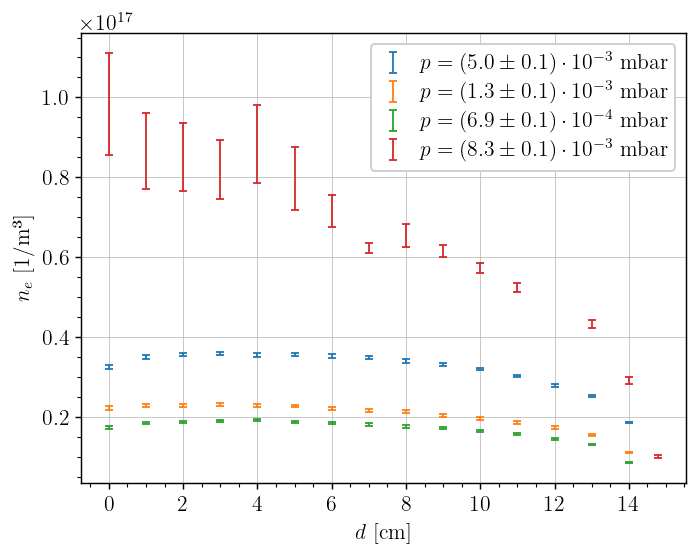
\includegraphics[width=4cm]{../figures/density_position.png}} % Title logo

\begin{document}

\begin{frame}
    \titlepage
\end{frame}

\begin{frame}{What is plasma?}{A subtitle about plasma}
    \begin{itemize}
    \item Tizio
    \item Caio
    \item Sempronio
    \end{itemize}
\end{frame}

\begin{frame}[plain]{Ciao}
When you want to hide the footer for dramatic effect.
\end{frame}


\begin{frame}{Some other stuff about Plasma}
    \begin{columns}[T]
        \column{0.6\textwidth}
        \centering
        This is column one with 75\% text width.

        \column{0.4\textwidth}
        \centering
        This is column two with 25\% text width.
        % \vspace{5cm}
        % And something in the bottom right corner.
    \end{columns}
\end{frame}

\begin{frame}{Some other stuff about Plasma}{Now with lines!}
    \begin{columns}
    % Column 1
    \begin{column}{0.49\textwidth}
        \begin{itemize}
            \item Mmmh yes the plasma is made of plasma
            \item Second smart remark
            \item Third smart remark
        \end{itemize}
    \end{column}
   % Column 2 (vertical line)
    \begin{column}{.02\textwidth}
        \rule{.1mm}{0.7\textheight}
    \end{column}
   % Column 3    
    \begin{column}{0.49\textwidth}
        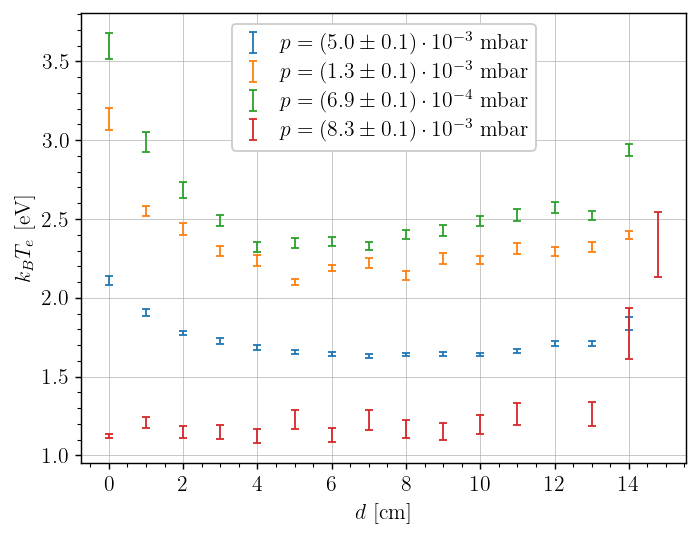
\includegraphics[width=\textwidth]{../figures/temperatureeV_position.png}
    \end{column}
    \end{columns}
\end{frame}

\begin{frame}{On the thermal properties of plasma}
    \begin{block}{Caution!}
        Plasma is hot
    \end{block}
\end{frame}

\begin{frame}{Overlays in Beamer}
    The easiest way is to use the stop command
    \pause

    Like this
    \pause

    There are other very customisable ways but we won't need them.
\end{frame}

\begin{frame}[fragile]{Beamer Font family}
    \verb|\rmfamily|: \rmfamily CM Roman

    \verb|\sffamily|: \sffamily CM Sans serif

    \verb|\ttfamily|: \ttfamily CM Typewriter

    some math: $y = f(x)$
\end{frame}

\end{document}